\documentclass{article}
\usepackage{graphicx}
\pagestyle{empty}
\topmargin -1 cm
\textheight=9.0in

\begin{document}

(I changed the value of $\Gamma_h$, because I think that the width of
the mass resonance is relevant in determining the width of the shell
of momentum integration.  My assumtion is that momentum is integrated
over all $\vec{p}_Z$ and all $\vec{p}_H$ with a weighting factor that
makes only states with $\vec{p}_Z + \vec{p}_H$ near
$\vec{p}_{e^+} + \vec{p}_{e^-}$ relevent.  When I took field theory,
the final states were always stable particles, so this weighting
factor was a delta function.  If there's a spread in Higgs mass values
(albeit a small one), this shell in \{$\vec{p}_Z$, $\vec{p}_H$\} space
can have some thickness (albeit not very much), and this thickness
scales with $\Gamma_H$.

Aha!  {\bf the Higgs width doesn't matter,} because even though the
momentum-integration shell has a width related to $\Gamma_H$, the
weighting distribution is normalized.  A non-zero $\Gamma_H$ only
widens the spread of \{$\vec{p}_Z$, $\vec{p}_H$\} values sampled by
the integration, it doesn't change their overall contribution.  I
expect the matrix element to scale very slowly with
\{$\vec{p}_Z$, $\vec{p}_H$\} compared to $\Gamma_H$.)

\begin{center}
  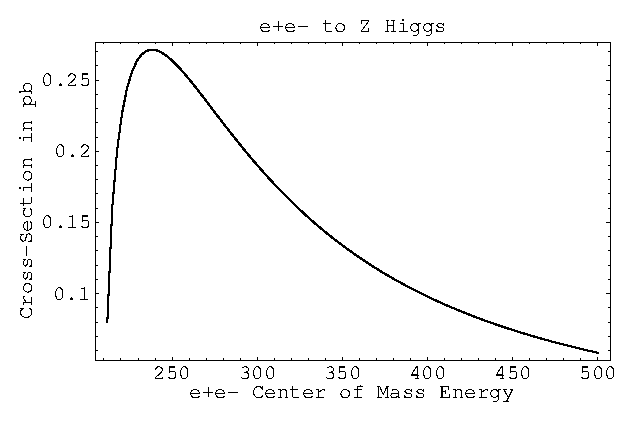
\includegraphics[width=\linewidth]{prod_zh.eps}
\end{center}

Now, you may be wondering why I only have a two-body final state on
this plot.  It's the only one calculable with Simpson's rule.  I
created a {\tt n\_comphep} for the other final states, and used Vegas
to plot some distributions, but if you want a distribution of
cross-section dependence on beam energy, you will get a histogram with
only one bin filled.  Vegas generates all events with only the given
beam energy.

This is a reasonable enough thing to do--- if you could change it.
The easiest way I can see to change the beam energy is to escape out
to the ``IN state'' menu, change both beam energies, go back to Vegas,
``start integration'' again, and then read the new total cross-section
off of the screen.  It was bad enough having to waddle through the
menu system eight times to make the branching fractions plot, I'm not
going to do it hundreds of times!

Then I tried everything I could think of to automate the process.  I
looked at the {\tt n\_comphep} code to see if I could just find the
function it calls to get a cross-section, link that into a new C
program and run it many times with my choice of input parameters.  But
the code is autogenerated and I couldn't make any sense of it
whatsoever.  Then I tried the {\tt -blind} option--- maybe I could
make an elaborate key sequence to get one datapoint to a file, so that
I could make that into a huge shell script and run it as a batch
process.  But the {\tt -blind} option {\it always} led to an immediate
segmentation fault.  Finally, I looked in the manual, the
``up-to-date'' one that came with my version 4.4 CompHEP, and there
was a whole section on running Vegas as a batch process (``because the
user interface has not yet been written.''  Hmmm).  None of that
section is applicable anymore--- no files are generated named
{\tt events\_1} (or anything like that), there's no executable
{\tt getEvents}, and passing the same kind of text file to the
executable which {\it is} generated doesn't do anything at all.  I
downloaded an older version of CompHEP--- version 4.2--- and had
exactly the same problems.

So it looks like they once provided a function which calculated
cross-sections from arbitrary inputs.  Now they have a graphical user
interface that lets you plot some things--- the things they thought
you might like to see.  This has been a constant source of aggravation
to me since 1990.

Since the order of magnitude might be useful, here are the other two
production cross-sections at a center of mass of 350 GeV:
\begin{center}
  \begin{tabular}{c p{2 cm} c}
    $e^+e^- \to e^+e^-h$ & & $8.002 \times 10^{-3}$ \\
    $e^+e^- \to \nu\bar{\nu}h$ & & $4.035 \times 10^{-2}$
  \end{tabular}
\end{center}


\end{document}
